% Theorem 3.1 (posterior consistency) + assumptions A1 & A2 --- deep-dive deck.
% Standalone mini-deck, same metropolis style as ../presentation.tex.
% Build with: make   (latexmk + lualatex)
\documentclass[aspectratio=169,10pt]{beamer}

\usetheme{metropolis}
\metroset{progressbar=frametitle, numbering=fraction, block=fill}

\usepackage[T1]{fontenc}
\usepackage{booktabs}
\usepackage{amsmath,amssymb}
\usepackage{tikz}
\usetikzlibrary{positioning,arrows.meta,fit,backgrounds,calc,matrix}
\usepackage{xcolor}

% --- palette (identical to the main deck) ----------------------------------
\definecolor{accent}{HTML}{C1121F}
\definecolor{ink}{HTML}{2B2D42}
\definecolor{muted}{HTML}{6C757D}
\definecolor{good}{HTML}{2A9D8F}
\setbeamercolor{frametitle}{bg=ink}
\setbeamercolor{background canvas}{bg=white}
\setbeamercolor{normal text}{fg=ink, bg=white}
\setbeamercolor{progress bar}{fg=accent}
\setbeamercolor{alerted text}{fg=accent}

\newcommand{\hl}[1]{{\color{accent}\textbf{#1}}}
\newcommand{\gd}[1]{{\color{good}\textbf{#1}}}
\newcommand{\mut}[1]{{\color{muted}#1}}
\newcommand{\cit}[1]{{\scriptsize\color{muted}[#1]}}

% reusable model-space blob (support P)
\def\Pblob{plot[smooth cycle, tension=0.8] coordinates
  {(0,0) (1.4,-0.2) (2.7,0.2) (2.9,1.2) (2.0,2.0) (0.7,1.9) (-0.4,1.0)}}

\title{When can the PPD learn?}
\subtitle{Posterior consistency \& its assumptions A1 \& A2 \;\cit{Nagler '23, Thm 3.1}}
\author{\underline{Gurmeher} Singh Puri \;\&\; Salih \underline{Bora} Öztürk}
\institute{Group 4 \;\textperiodcentered\; FM4SD Seminar \;\textperiodcentered\; SS26}
\date{}

\begin{document}

\maketitle

% ===========================================================================
% 1. The claim + the shape of the argument
% ===========================================================================
\begin{frame}[t]{The claim: the target really does learn \cit{Thm 3.1}}

  \onslide<1->{\centering
    Under assumptions \hl{A1} and \hl{A2}, there is a $p^*\in\mathcal P$ with
    \[
      \pi(y\mid x,\mathcal D_n)\ \xrightarrow[\;n\to\infty\;]{}\ p^*(y\mid x)
      \quad\text{almost surely,}
    \]
    and $p^*$ is the \hl{KL-optimal} approximation of the truth $p_0$ inside $\mathcal P$.\par}
  \vspace{1.0em}

  \onslide<2->{\centering It's a race with a finish line:\par}
  \vspace{0.4em}
  \begin{columns}[T]
    \column{0.5\textwidth}
      \onslide<2->{\begin{block}{A1 --- the finish line exists}
        \footnotesize a \emph{unique}, finite-distance best in-support model $p^*$ to converge to.
      \end{block}}
    \column{0.5\textwidth}
      \onslide<3->{\begin{block}{A2 --- the runner reaches it}
        \footnotesize the prior is well-behaved enough that the posterior actually \emph{contracts} onto $p^*$.
      \end{block}}
  \end{columns}
  \vspace{0.8em}

  \onslide<4->{\centering
    {\footnotesize\mut{Crucial: this is about the \hl{PPD} --- the \emph{target} --- not the frozen network $q_{\hat\theta}$.}}\par}
\end{frame}

% ===========================================================================
% 2. Setup: the prior's vocabulary, and p* as a KL projection
% ===========================================================================
\begin{frame}[t]{The setup: the prior's vocabulary}

  \onslide<1->{\centering
    The prior $\Pi$ only ``believes in'' some distributions --- its \hl{support}
    $\mathcal P=\{p:\Pi(p)>0\}$. The truth $p_0$ \emph{need not be inside it}.\par}
  \vspace{0.4em}

  \begin{columns}[T]
    \column{0.55\textwidth}
      \onslide<1->{\centering
      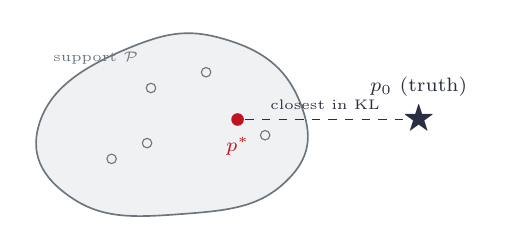
\begin{tikzpicture}[>=Latex]
        \fill[muted!10] \Pblob;
        \draw[muted, line width=0.6pt] \Pblob;
        \node[muted, font=\tiny] at (0.3,1.78){support $\mathcal P$};
        % a few supported models
        \foreach \m in {(0.5,0.5),(1.0,1.4),(0.95,0.7),(1.7,1.6),(2.45,0.8)}
          \draw[muted] \m circle(0.06);
        % p* = KL-closest in-support model
        \fill[accent] (2.1,1.0) circle(0.08);
        \node[accent, font=\scriptsize, below=0pt] at (2.1,0.9){$p^*$};
        % truth outside
        \node[ink] at (4.4,1.0) {\large$\bigstar$};
        \node[ink, font=\scriptsize] at (4.4,1.42){$p_0$ (truth)};
        \draw[ink, dashed] (2.2,1.0) -- (4.22,1.0)
          node[midway, above, font=\tiny]{closest in KL};
      \end{tikzpicture}}
    \column{0.45\textwidth}
      \onslide<2->{%
        $p^*$ is the in-support model \hl{closest to $p_0$} in KL:
        \[ p^*=\arg\min_{p\in\mathcal P}\ \mathrm{KL}(p\,\|\,p_0). \]
        \par}
      \medskip
      \onslide<3->{{\footnotesize\mut{\textbf{Example.} Prior supports only logistic-\emph{linear}
        models, but $p_0$ is wiggly. Then $p^*$ is the \hl{best linear fit} ---
        the best the prior \emph{can} express.}}\par}
  \end{columns}
  \vspace{0.5em}

  \onslide<3->{\centering
    {\footnotesize\gd{So convergence is to the best the prior can do} ---
    \mut{$p^*=p_0$ only when the truth happens to be in support.}\par}}
\end{frame}

% ===========================================================================
% 2b. What "KL-optimal" means
% ===========================================================================
\begin{frame}[t]{What does ``KL-optimal'' mean?}

  \onslide<1->{\centering
    The \hl{Kullback--Leibler divergence} measures how far a model $p$ is from the truth $p_0$:
    \[ \mathrm{KL}(p\,\|\,p_0)=\mathbb{E}_{p}\!\Big[\log\tfrac{p}{p_0}\Big]\ \ge 0,
       \qquad =0 \iff p=p_0. \]
    {\footnotesize\mut{a ``distance'' between distributions --- the \emph{log-loss} currency.}}\par}
  \vspace{0.3em}

  \onslide<2->{\centering
    \textbf{KL-optimal} $p^*$ $=$ the in-support model that minimizes it:
    \[ p^*=\arg\min_{p\in\mathcal P}\ \mathrm{KL}(p\,\|\,p_0)
       \quad\text{\footnotesize\mut{$=$ best impersonation of $p_0$ the prior can express.}} \]\par}
  \vspace{0.2em}

  \onslide<3->{\centering
    \textbf{Why KL?} The PFN is \emph{trained} to maximize log-likelihood $\mathbb{E}_\Pi[\log q]$ \cit{Thm 2.1},
    and maximizing log-likelihood $\Longleftrightarrow$ minimizing KL.\\[2pt]
    {\footnotesize\gd{So ``KL-optimal'' $=$ best in exactly the currency the network optimizes.}}\par}
  \vspace{0.2em}

  \onslide<4->{\centering
    {\footnotesize\mut{Intuition: KL $=$ the \emph{extra surprise} (excess log-loss) from using $p$ instead of $p_0$;
    $p^*$ leaves you \hl{least surprised} on average.}}\par}
\end{frame}

% ===========================================================================
% 3. A1 --- the target
% ===========================================================================
\begin{frame}[t]{A1 --- a well-defined finish line}

  \onslide<1->{\centering
    \emph{There is a \hl{unique} $p^*\in\mathcal P$ minimizing $\mathrm{KL}(p\,\|\,p_0)$,
    with $\mathrm{KL}(p^*\,\|\,p_0)<\infty$.}\par}
  \vspace{0.9em}

  \onslide<2->{\centering Two clauses --- each kills one disaster:\par}
  \vspace{0.4em}

  \onslide<2->{\centering
  \begin{tabular}{@{}p{0.30\textwidth} p{0.60\textwidth}@{}}
    \toprule
    \textbf{Clause} & \textbf{Disaster it prevents} \\
    \midrule
    \hl{unique} $p^*$ & two equally-close models $\Rightarrow$ posterior \emph{ping-pongs}
      between them, never settles $\Rightarrow$ no single limit. \\[0.7em]
    $\mathrm{KL}(p^*\|p_0)<\infty$ & even the \emph{best} fit infinitely far from $p_0$
      $\Rightarrow$ prior is in the wrong universe; ``best approximation'' is meaningless. \\
    \bottomrule
  \end{tabular}\par}
  \vspace{0.9em}

  \onslide<3->{\centering
    {\gd{A1's whole job:}} make the sentence ``the PPD converges to the \emph{best the prior can do}''
    \hl{point at a real, unique object}.\par}
\end{frame}

% ===========================================================================
% 4a. A2 --- the terrain (the pieces / glossary)
% ===========================================================================
\begin{frame}[t]{A2 --- the prior must be well-behaved: the pieces}

  \onslide<1->{\centering
    A1 gives a finish line; it does \emph{not} guarantee anyone reaches it ---
    a too-diffuse prior leaves the posterior \hl{smeared forever}.\par}
  \vfill

  \begin{columns}[c]
    \column{0.42\textwidth}
      \onslide<2->{\centering
      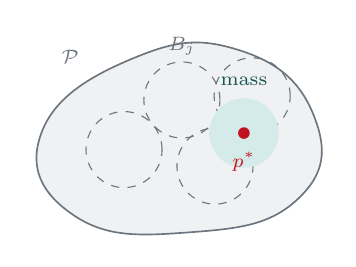
\begin{tikzpicture}[>=Latex, scale=1.05]
        \fill[muted!10] \Pblob;
        \draw[muted, line width=0.6pt] \Pblob;
        \foreach \c in {(0.6,0.8),(1.3,1.4),(1.7,0.6),(2.15,1.45)}
          \draw[muted, dashed, line width=0.4pt] \c circle(0.46);
        \fill[good!20] (2.05,1.0) circle(0.42);
        \fill[accent] (2.05,1.0) circle(0.07);
        \node[accent, font=\scriptsize, below=1pt] at (2.05,0.92){$p^*$};
        \node[muted, font=\scriptsize] at (-0.05,1.92){$\mathcal P$};
        \node[muted, font=\scriptsize] at (1.30,2.05){$B_j$};
        \node[good!55!black, font=\scriptsize] at (2.05,1.62){mass};
      \end{tikzpicture}}
    \column{0.54\textwidth}
      \onslide<2->{\small
      \begin{tabular}{@{}r@{\ \ }l@{}}
        {\color{accent}$\mathcal P$}  & the prior's possible models \\[0.7em]
        {\color{accent}$B_j$}         & a \emph{bin} of similar models \\[0.7em]
        {\color{accent}$J(\alpha)$}   & the number of bins (finite) \\[0.7em]
        {\color{accent}$H(p,p')$}     & Hellinger distance between models \\[0.7em]
        {\color{accent}$\Pi(B_j)$}    & prior mass in bin $j$ \\
      \end{tabular}}
  \end{columns}
  \vfill
\end{frame}

% ===========================================================================
% 4b. A2 --- what is alpha + the three demands
% ===========================================================================
\begin{frame}[t]{A2 --- what is $\alpha$, and the three demands}

  \onslide<1->{\centering
    $\alpha\in(0,\tfrac12)$ is a \hl{resolution / strictness dial} --- not a probability or a rate ---
    and A2 must hold \hl{for every} $\alpha$.\\[2pt]
    {\footnotesize\mut{smaller $\alpha$ $=$ stricter: finer bins \emph{and} a tighter bound on the mass.}}\par}
  \vfill

  \onslide<2->{\centering For each $\alpha$, cover $\mathcal P$ with finitely many bins so that:\par}
  \medskip
  \onslide<2->{\centering
    \textbf{1.\ Cover}\;\; $\mathcal P\subseteq\bigcup_j B_j$
      \;\;{\footnotesize\mut{(every model in some bin)}}\\[8pt]
    \textbf{2.\ Tiny bins}\;\; $\displaystyle\sup_{p,p'\in B_j}H(p,p')\le 4(\alpha^2/2)^{1/\alpha}$
      \;\;{\footnotesize\mut{(shrinks as $\alpha\downarrow$)}}\\[8pt]
    \textbf{3.\ Summable mass}\;\; $\textstyle\sum_j \Pi(B_j)^\alpha<\infty$
      \;\;{\footnotesize\mut{(not too many bins)}}\par}
  \vfill

  \onslide<3->{\centering
    {\footnotesize Condition \textbf{3} is the engine: since $\alpha<\tfrac12$, $x^\alpha$ decays \emph{slowly},
    so a prior smeared over endlessly many models blows the sum up.}\\[2pt]
    {\footnotesize\gd{controlled support $\Rightarrow$ posterior contracts onto $p^*$.}}\par}
  \vfill
\end{frame}

% ===========================================================================
% 5. A1 + A2 together -> posterior consistency -> the pivot
% ===========================================================================
\begin{frame}[t]{A1 $+$ A2 $\Rightarrow$ posterior consistency}

  \onslide<1->{\centering
  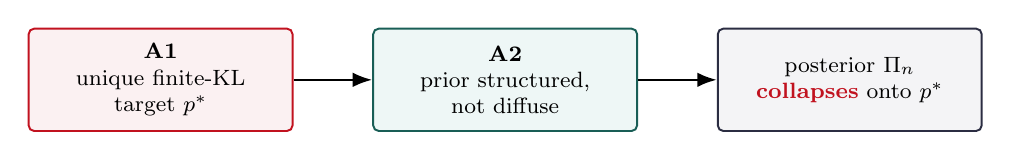
\begin{tikzpicture}[>=Latex, font=\footnotesize,
      box/.style={rounded corners=2pt, draw, line width=0.7pt, align=center,
                  inner sep=5pt, minimum height=13mm, text width=30mm}]
    \node[box, draw=accent, fill=accent!6] (a1) {\textbf{A1}\\ unique finite-KL\\ target $p^*$};
    \node[box, draw=good!60!black, fill=good!8, right=10mm of a1] (a2)
        {\textbf{A2}\\ prior structured,\\ not diffuse};
    \node[box, draw=ink, fill=ink!5, right=10mm of a2] (post)
        {posterior $\Pi_n$\\ \hl{collapses} onto $p^*$};
    \draw[->, line width=0.9pt] (a1) -- (a2);
    \draw[->, line width=0.9pt] (a2) -- (post);
  \end{tikzpicture}}
  \vspace{0.5em}

  \onslide<2->{\centering
    The PPD is the \hl{posterior mean}, so the collapse carries straight through:
    \[
      \pi(y\mid x,\mathcal D_n)=\int p(y\mid x)\,d\Pi_n(p)
      \ \xrightarrow[\;\Pi_n\to\delta_{p^*}\;]{}\ p^*(y\mid x).
    \]\par}
  \vspace{0.4em}

  \onslide<3->{\centering
    {\footnotesize\mut{Drop A1 $\to$ no unique/finite destination.\quad
      Drop A2 $\to$ destination exists, but the posterior may never get there.}}\par}
  \vspace{0.7em}

  \onslide<4->{\centering
    \hl{The pivot:} all of this is about the \hl{PPD} (the target).
    The frozen $q_{\hat\theta}$ is \emph{not} a PPD past its trained sizes ---
    \gd{so the next section switches to a frequentist lens.}\par}
\end{frame}

\end{document}
